
\DocumentMetadata{
	lang		= eng-US, 	% default
	pdfstandard	= A-3u,		% A-2b, A-2u, A-3b, A-3u. Check that your figures also meet the standard you choose.
	pdfversion	= 1.7, 		% an older version of PDF, but very widely supported
%	pdfversion  = 2.0, 		% default for LaTeX. Version 2.0 supports tagged PDF.
%	pdfstandard = { ua-2 , a-4f }, % run with lualatex and use a very recent LaTeX format (e.g., 2025/11/01)
%	tagging 	= on, 		% for producing tagged pdf
}

%%%%%%%%%%%%%%%%%%%%%%%%%%%%%%%%%%%%%%%%%%%%%%%%%%%%%%%%%%%%%%%%%%%%%%%%%%%%%%%%%%%%%%%%%%%%%%%%%%%%%%%

%% CLASS OPTIONS are described above. Change the options given below to meet your needs.
%% 
%%	 	NB: Remove the [colorlinks] option before *final* submission to ASME, to get black text for printing,
%%			but keep that option for electronic use.
%%
%%		NB: If you are not using the language options, * remove * them (together with Appendices C and D).
%%			Greek, cyrillic languages, and vietnamese if used, must be named as \documentclass options under pdftex.
%%			Spanish, german, and many others, if used, do not need to be named when the babel package is dated 2024 or later.
%%
%%		NB: the mathalfa option was dropped in v1.41; load the mathalpha package in your preamble instead.

\documentclass[colorlinks,upint,subscriptcorrection,varvw,hyphenate,balance,greek,russian,vietnamese,german]{asmeconf} % pdftex

%\documentclass[colorlinks,upint,subscriptcorrection,varvw,balance,loadscripts,german,vietamese]{asmeconf} % lualatex

%%%%%  pdf metadata  %%%%%%%%%%%%%%%%%%%%%%%%%%%%%%%%%%%%%%%%%%%%%%%%%%%%%%%%%%%%%%%%%%%%%%%%%%%%%%%%%%

\hypersetup{%
	pdfauthor={Amal Chulliyat Jose and Georgios Katranis and Andrey Morozov},									  
	pdftitle={Probabilistic Action Prediction of Human Drivers Using Dynamic Bayesian Networks},                  
	pdfkeywords={human driver behavior modeling, maneuver prediction, dynamic Bayesian networks, highD, probabilistic modeling},
	pdfsubject = {ASME IMECE2026 conference paper},			  
}
% If an author name or the title include a comma, enclosed it in braces, e.g., pdfauthor{John Forbes Nash{,} Jr.}


%%%%%%%%%%%%%%%%%%%%%%%%%%%%%%%%%%%%%%%%%%%%%%%%%%%%%%%%%%%%%%%%%%%%%%%%%%%%%%%%%%%%%%%%%%%%%%%%%%%%%%%

\allowdisplaybreaks % from amsmath package, allows multiline equations to break across pages (delete if not wanted)
					% using \\* instead of \\ will prevent specific lines from being pagebreaks.

% logos used in this document
\newcommand*\pdfTeX{pdf\TeX}    
\newcommand*\LuaLaTeX{Lua\LaTeX}
\newcommand*\BibTeX{Bib\TeX}

\begin{document}

\ConfName{Proceedings of the ASME 2026\linebreak International Mechanical Engineering Congress and Exposition}
\ConfAcronym{IMECE2026}
\ConfDate{November 8--12, 2026} 
\ConfCity{Vancouver, British Columbia, Canada}
\PaperNo{IMECE2026-192718}


\title{Probabilistic Action Prediction of Human Drivers Using Dynamic Bayesian Networks} 
 
\SetAuthors{
    Amal Chulliyat Jose\affil{}, 
	Georgios Katranis\affil{}\CorrespondingAuthor{georgios.katranis@ias.uni-stuttgart.de}, 
	Andrey Morozov\affil{}
	}

\SetAffiliation{}{University of Stuttgart, Germany}

\maketitle


\keywords{Human Driver Behavior Modeling, Autonomous Driving, Human-Driven Vehicles, Dynamic Bayesian Networks, Maneuver Prediction, Probabilistic 
Modeling, Mixed Traffic Environments}


%%%%%  ABSTRACT  %%%%%%%%%%%%%%%%%%%%%%%%%%%%%%%%%%%%%%%%%%%%%%%%%%%
\begin{abstract}
For the foreseeable future, autonomous vehicles (AVs) will have to operate in mixed traffic with human-driven vehicles (HDVs), which requires reliable prediction of human maneuvers.  
This paper presents an interpretable probabilistic framework for short-horizon human driver maneuver prediction using Dynamic Bayesian Networks (DBNs). 
The model is trained on the highD naturalistic highway dataset using window-based observations from vehicle motion and surrounding traffic interactions. 
The model uses a hierarchical latent structure in which action states are conditioned on broader driving regimes, allowing maneuver type and interaction context to be represented jointly.

On the test set, the proposed model achieves 46.4\% exact next-step accuracy, 44.3\% macro precision, and a 55.2\% hit rate over a 2\,s prediction horizon. 
When semantically similar maneuver classes are grouped, performance increases to 62.4\% exact next-step accuracy and a 70.2\% horizon hit rate. 
This suggests that many prediction errors are near-misses between related actions. 
The average CPU latency for online belief update and next-maneuver prediction for a single vehicle 
was 0.164\,ms, which is well below the 400\,ms interval between consecutive inputs. 
These results show that DBNs can learn meaningful temporal behavior patterns and support fast, interpretable short-horizon maneuver prediction.

\end{abstract}


%%%%%%%%%  BODY OF PAPER %%%%%%%%%%%%%%%%%%%%%%%%%%%%%%%%%

\section{Introduction}
Recent progress in artificial intelligence (AI), sensing, computing, and communication has accelerated the development of AVs. 
However, safe operation still depends on how well AVs can handle mixed traffic with HDVs, since fully autonomous traffic systems do not yet exist.

In mixed traffic, an AV cannot directly observe the intentions of nearby HDVs. Instead, human driver behavior must be inferred from observable 
cues such as vehicle motion, lane changes, relative positions, and interactions with other nearby vehicles \cite{Schwarting2018}.
Human driver behavior prediction is therefore an important problem in autonomous driving. Estimating likely future maneuvers can support downstream 
tasks such as risk assessment, trajectory prediction, and motion planning \cite{Lefevre2014,Madjid_2026,Schwarting2018}.

Existing behavior prediction methods include rule-based, probabilistic, and learning-based approaches \cite{10054035,Rudenko_2020,Lefevre2014}. 
Rule-based models are simple and interpretable but often too rigid to capture the variability of real human behavior. Learning-based methods can 
learn complex patterns from large datasets, but many are difficult to interpret and are often treated as black boxes. 
Probabilistic models provide a useful middle ground because they can represent uncertainty, capture temporal dependencies, and remain interpretable.

This paper focuses on probabilistic modeling of high-level human driving behavior in highway traffic, with the goal of predicting likely future maneuvers 
of surrounding drivers while explicitly representing uncertainty. 
In the proposed framework, future maneuvers are represented as discrete action states, and a DBN models the temporal relationship between trajectory-based 
observations and hidden behavioral states. 
Driver intent is represented through latent variables and inferred probabilistically from observed vehicle motion and traffic context \cite{murphy2002dynamic}. 
The model is trained and evaluated on the highD dataset \cite{krajewski2018highddatasetdronedataset} using features that describe vehicle motion, 
surrounding traffic context, and interaction behavior.

The study evaluates whether this framework can provide accurate, interpretable, and computationally 
efficient short-horizon predictions of future human driving maneuvers.

The main contributions of this paper are threefold: 
(1) a structured DBN framework for probabilistic short-horizon maneuver prediction with interpretable latent states, 
(2) a window-based observation design that combines ego motion with surrounding traffic interaction features, and 
(3) an evaluation on the highD dataset covering predictive accuracy, short-horizon hit rate, and online inference latency.

%%%%%%%%%%%%%%%%%%%%%%%%%%%%%%%%%%%%%%%%%%%%%%%%%%%%%%%%%%%

\section{Related Work}
Human driver behavior and maneuver prediction methods are commonly grouped into rule-based, probabilistic, and learning-based approaches, 
which differ in how they represent driver decisions, uncertainty, and temporal dependencies.  

\subsection{Driver Behavior and Maneuver Prediction Approaches}
Rule-based models describe driving behavior through explicit mathematical equations or logical rules. 
Typical examples include car-following and lane-change models such as the Intelligent Driver Model (IDM), Gipps' model and the Minimizing Overall Braking Induced by 
Lane Changes (MOBIL) model, 
which relate observable traffic variables to 
longitudinal or lateral driving actions \cite{PhysRevE.62.1805,Kesting2007GeneralLM,zhou2025,GIPPS1981105}. 
Their main strengths are interpretability, low computational cost, and clear physical meaning of parameters. 
However, they usually rely on hand-crafted assumptions and often represent driver behavior in a simplified or mostly deterministic way. 
This limits their ability to capture uncertainty and variability across drivers in real traffic. 

Probabilistic models address this limitation by describing driver behavior as a stochastic process. 
Instead of predicting a single fixed response, they represent multiple possible behaviors and quantify uncertainty over future 
actions \cite{wang2023probabilisticpredictionlongitudinaltrajectory}. 

Learning-based methods form another major family of behavior prediction models. 
Classical machine learning methods such as Support Vector Machine (SVM), decision trees, and random forests were early data-driven approaches for intent 
recognition and maneuver classification \cite{app112210562}. 
More recent deep learning models can learn complex nonlinear patterns directly from large-scale driving data and often achieve strong 
predictive performance. 
However, they are usually less interpretable and often need larger datasets and more careful tuning than structured probabilistic models.


\subsection{Probabilistic Temporal Models}
Among probabilistic methods, Hidden Markov Models (HMMs) are a common starting point for modeling time-varying driving behavior. 
They represent behavior as a sequence of latent states that generate observable signals \cite{rabiner1989tutorial}. 
In driver modeling, these hidden states can correspond to maneuver-related modes such as lane keeping, braking, or overtaking \cite{8500717}. 
HMMs are attractive because of their simple structure and efficient inference. 
However, they represent the hidden state with a single variable, which limits how much structure can be encoded in the model.

DBNs extend this idea by allowing the latent and observed state to be represented in factored form across time \cite{murphy2002dynamic,pearl1995bayesian}. 
Compared with HMMs, they can model richer dependencies between hidden variables, observations, and temporal transitions. 
This added flexibility makes DBNs well suited for driver behavior analysis, especially when the goal is to separate different aspects of behavior while 
preserving a probabilistic and interpretable representation. 
Prior work has used Bayesian-network-based models to represent causal relations in driver behavior and to support lane-change reasoning and safety-related 
inference \cite{electronics8010040,2025bayesiannetworkapproachbuilding,talluri2025enhancingsafetystandardsautomated}.

Other probabilistic approaches, including Gaussian-based models such as Gaussian Mixture Model (GMM), Gaussian Mixture Regression (GMR), and Gaussian Process Regression (GPR), 
are often used to model continuous driving quantities 
such as acceleration or trajectory evolution \cite{mozaffari2023multimodalmanoeuvretrajectoryprediction,zhang2024learningcarfollowingbehaviorsusing,Bethge2023ModelPC}. 


\subsection{Learning-Based Prediction Models}

Deep learning  has become a major direction in trajectory and maneuver prediction. Recurrent Neural Networks 
(RNNs) and Long Short-Term Memory (LSTM) networks were widely used to model temporal dependencies in driving sequences, while Graph Neural Networks (GNNs) were later introduced 
to better represent 
interactions between multiple traffic participants \cite{Goodfellow-et-al-2016,salzmann2021trajectrondynamicallyfeasibletrajectoryforecasting}. 
More recently, Transformer-based models have shown strong performance by capturing long-range dependencies and multi-agent interactions through attention 
mechanisms \cite{vaswaniattention,ngiam2022scenetransformerunifiedarchitecture,shi2023motiontransformerglobalintention,inproceedingshivt}. 
Generative approaches such as Conditional Variational Autoencoder (CVAE) and diffusion models further support multimodal prediction by generating multiple plausible future trajectories 
under the same observed context 
\cite{NIPS2015_8d55a249,salzmann2021trajectrondynamicallyfeasibletrajectoryforecasting,mangalam2020journeydestinationendpointconditioned,ho2020denoisingdiffusionprobabilisticmodels,jiang2023motiondiffusercontrollablemultiagentmotion}.

Although these methods are powerful, most of them mainly target trajectory forecasting and often operate as highly data-driven black-box models. 
For applications where uncertainty representation, temporal structure, and behavioral interpretability are important, this can be a limitation. 
In particular, it is often harder to connect their internal representations to semantically meaningful driver behavior modes or to use them directly in interpretable 
probabilistic reasoning.

\subsection{Positioning of This Work}

The review above shows a trade-off between simplicity, predictive power, and interpretability. 
Rule-based models are transparent but limited in uncertainty representation. 
Deep learning models are powerful but often difficult to interpret. 
Probabilistic temporal models, especially DBNs, offer a useful middle ground because they can represent uncertainty explicitly, model temporal evolution, 
and preserve a structured latent representation.

Motivated by this gap, this paper uses a DBN for probabilistic short-horizon prediction of human driver maneuvers in highway traffic. 
The model is designed to capture temporal behavior patterns through interpretable latent states while remaining suitable for online probabilistic inference. 
The work therefore focuses on structured behavior modeling and maneuver prediction of HDVs rather than full trajectory generation or downstream planning.


\section{Methodology}
This section presents the proposed framework for probabilistic short-horizon maneuver prediction of human-driven vehicles in highway traffic. 
Starting from raw trajectories in the highD dataset, the pipeline constructs a consistent vehicle-centric representation, extracts motion and interaction features, 
summarizes them over short sliding windows, and models the resulting observation sequences using a DBN. 
An overview of the full pipeline is shown in Fig.~\ref{fig:proposed_framework}.

\begin{figure}[t]
\centering
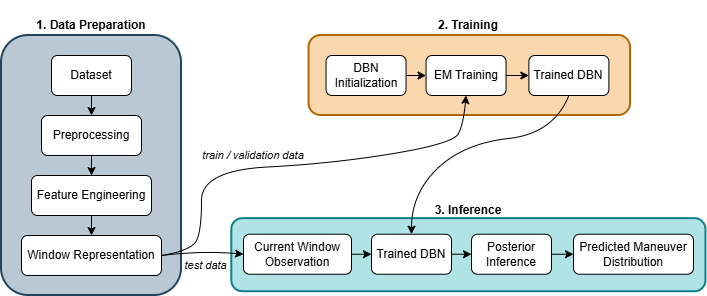
\includegraphics[width=\linewidth,
alt={Overview of the proposed framework, showing preprocessing of highD trajectories, window-based observation construction, DBN modeling, and short-horizon maneuver prediction.}]
{Framework.drawio.png}
\caption{Overview of the proposed framework}
\label{fig:proposed_framework}
\end{figure}

\subsection{Framework Overview}
The proposed framework consists of three main stages: preprocessing of raw trajectory data, 
probabilistic temporal modeling, and causal online prediction. 
First, frame-level trajectories from highD are converted into a consistent representation that is independent of the original driving direction. 
Next, ego-motion, lane-related, interaction, and risk-related features are extracted and aggregated over short overlapping windows. 
Each window then forms one observation for the DBN, which models temporal evolution through two latent variables: a style state and an action state. 
After training, the model is used for online filtering and one-step-ahead maneuver prediction.

\subsection{Dataset and Preprocessing}
The method is evaluated on the highD dataset \cite{krajewski2018highddatasetdronedataset}, which contains naturalistic highway trajectories recorded 
from drone videos on German highways. 
In this work, the first 25 recordings with three lanes in each driving direction are used in order to maintain a more uniform road geometry and 
traffic setting across the selected subset. 
For each vehicle, the dataset provides frame-level position, velocity, acceleration, lane information, neighboring-vehicle identifiers, and traffic-safety indicators 
such as time headway (THW) and time to collision (TTC).

Because the selected recordings contain traffic moving in opposite roadway directions, the raw kinematic signals do not follow a consistent sign convention across all vehicles. 
A vehicle-centric normalization step is therefore applied so that the same maneuver is represented with the same sign convention regardless of the original travel direction. 
This produces a consistent frame-level representation for later feature extraction and windowization. 

\subsection{Window-Based Observation Design}
The observation vector combines ego-motion, lane-related, interaction, and risk-related information. 
It includes kinematic quantities such as longitudinal and lateral velocity and acceleration, lane-boundary distances, lane-change evidence, front-vehicle safety 
indicators, and selected relative features describing nearby traffic participants. 
These variables are designed to represent both the state of the ego vehicle and the surrounding traffic context relevant for maneuver prediction.

Rather than using individual frames directly, the model operates on short temporal windows. 
Each trajectory is converted into a sequence of overlapping windows with length $W=50$ frames and stride $S=10$ frames. 
Since the highD dataset is recorded at 25\,Hz, each window covers 2.0\,s of history and consecutive windows start every 0.4\,s. 
Each window is summarized into one observation vector using simple temporal aggregation functions, which provide a compact representation of recent motion 
and interaction history while keeping the observation space manageable. 
The resulting windowization process is illustrated in Fig.~\ref{fig:window_based_representation}.
\begin{figure}[t]
\centering
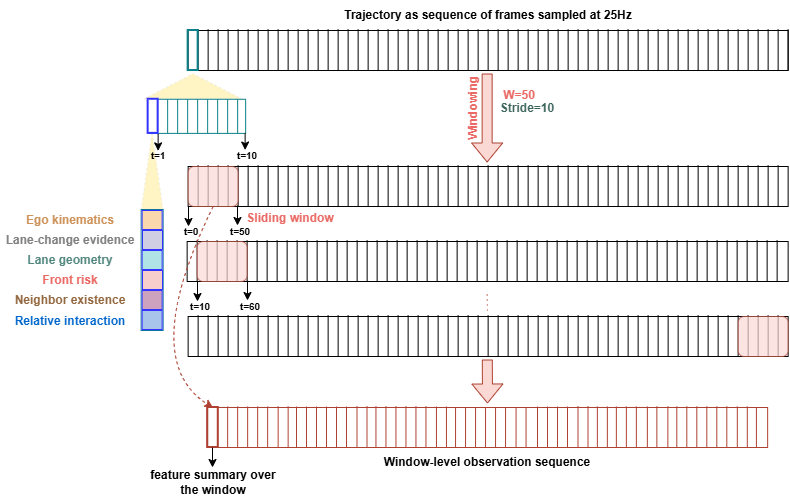
\includegraphics[width=\linewidth,
alt={Illustration of the window-based observation design. Raw frame-level trajectory features are grouped into overlapping temporal windows of length 50 
frames with stride 10 frames, and each window is summarized into one observation vector for the DBN.}]
{windowize.png}
\caption{Illustration of the sliding-window representation}
\label{fig:window_based_representation}
\end{figure}


\subsection{DBN Formulation}
The proposed DBN uses two discrete latent variables at each time step: a style state $S_t$ and an action state $A_t$. 
The style state captures a broader driving regime, while the action state represents the current maneuver. 
The observation vector $O_t$ corresponds to the aggregated window-level features described above. 
The graphical structure of the model is shown in Fig.~\ref{fig:proposed_dbn_structure}.
\begin{figure}[h]
\centering
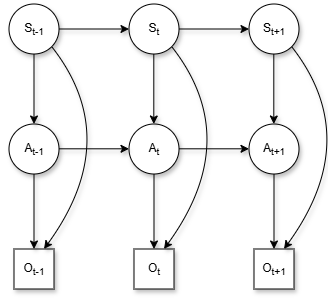
\includegraphics[width=0.55\linewidth,
alt={Factorized latent structure of the proposed DBN. The style state evolves over time, the action state depends on the previous action and current style state, 
and each observation depends on the latent state pair.}]
{DBN.drawio.png}
\caption{Structure of the proposed DBN}
\label{fig:proposed_dbn_structure}
\end{figure}

The temporal dependencies are factorized such that the style state evolves according to its previous value, while the action state depends on both the previous action 
and the current style. 
This structure reflects the assumption that the broader driving regime changes more slowly, whereas short-term maneuver depends on both recent behavior and current traffic context. 
The emission model links each window-level feature vector to the latent state pair $(S_t, A_t)$.

The joint distribution of the proposed DBN for a sequence of length $T$ is written as
\begin{equation}\label{eqn:dbn_factorization}
\begin{aligned}
&\Pr(S_{1:T},A_{1:T},O_{1:T}) \\
&= \Pr(S_1)\Pr(A_1 \mid S_1)\Pr(O_1 \mid S_1,A_1) \\
&\quad \times \prod_{t=2}^{T}
\Pr(S_t \mid S_{t-1})
\Pr(A_t \mid A_{t-1},S_t)
\Pr(O_t \mid S_t,A_t).
\end{aligned}
\end{equation}

The emission model is conditioned directly on the joint latent state pair $(S_t, A_t)$. 
Continuous features are modeled with diagonal Gaussian distributions and binary features with Bernoulli distributions. 

For each latent pair $(s,a)$, the emission likelihood is defined as
\begin{equation}\label{eqn:emission_model}
\begin{aligned}
\Pr(O_t \mid S_t=s,A_t=a)
&= \prod_{d \in \mathcal{C}}
\mathcal{N}\left(o_{t,d};\mu_{s,a,d},\sigma^2_{s,a,d}\right) \\
&\quad \times
\prod_{b \in \mathcal{B}}
\mathrm{Bern}\left(o_{t,b};\rho_{s,a,b}\right),
\end{aligned}
\end{equation}
where $\mathcal{C}$ is the set of continuous features and $\mathcal{B}$ is the set of binary features. 
The parameters $\mu_{s,a,d}$ and $\sigma^2_{s,a,d}$ define the Gaussian emission for continuous feature $d$, while $\rho_{s,a,b}$ 
defines the Bernoulli probability for binary feature $b$.

\subsection{Training and Online Prediction}
Model parameters are estimated from the training data using the expectation-maximization (EM) algorithm. 
Continuous features are standardized using statistics computed from the training split only, and model initialization includes initial-state probabilities, 
transition probabilities, and emission parameters derived from the training data. 
The training procedure learns both the temporal dynamics of the latent states and the emission model linking latent states to window-level features.

After training, the model is used in a causal online setting. 
At time step $t$, the filtered belief over the latent state pair is updated using the observations available up to that time, and the transition model is then used to obtain 
the one-step-ahead predictive distribution over future maneuvers. 
The causal prediction process is illustrated in Fig.~\ref{fig:predictive_evaluation_pipeline}.
\begin{figure}[h]
\centering
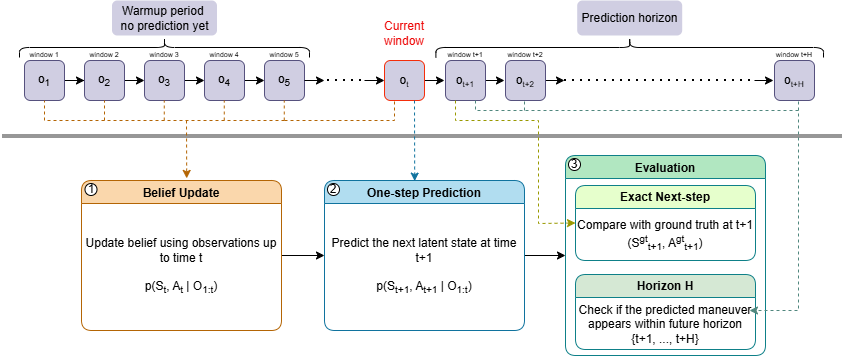
\includegraphics[width=\linewidth,
alt={Causal online prediction pipeline. Past observations are used to update the filtered belief over latent style and action states, and the transition model produces a one-step-ahead maneuver prediction.}]
{prediction.png}
\caption{Causal online prediction pipeline used for one-step-ahead maneuver prediction}
\label{fig:predictive_evaluation_pipeline}
\end{figure}

After filtering, the one-step-ahead predictive distribution over the next action is obtained as
\begin{equation}\label{eqn:action_prediction}
\Pr(A_{t+1} \mid O_{1:t})
=
\sum_{s_t,a_t,s_{t+1}}
\Pr(S_t=s_t,A_t=a_t \mid O_{1:t})
\Pr(S_{t+1} \mid s_t)
\Pr(A_{t+1} \mid a_t,S_{t+1}).
\end{equation}

\section{Experimental Setup}

\subsection{Data Split and Compared Configurations}
The selected highD subset is partitioned at the vehicle level into disjoint training, validation, and test sets to prevent leakage across overlapping 
windows from the same trajectory. 
The split contains 35{,}318 training vehicles (70\%), 5{,}045 validation vehicles (10\%), and 10{,}092 test vehicles (20\%). 
The training set is used for parameter estimation, the validation set is used for model selection and early stopping, and the test set is reserved for final evaluation.

\subsection{Evaluation Protocol}
Evaluation is performed in both generative and predictive settings. 
In the generative setting, the trained model is applied to full unseen test sequences to measure how well it explains the observation data. 
In the predictive setting, inference is carried out online in a strictly causal manner. 
At each time step, only observations available up to that time are used to update the filtered belief and generate a one-step-ahead maneuver prediction.

During online evaluation, the first five window observations of each test trajectory are used as warmup and are excluded from scoring. 
After warmup, one-step-ahead predictions are generated sequentially. 
For horizon-based evaluation, the forecast horizon covers the next five observations, corresponding to 2.0\,s.

\subsection{Evaluation Metrics}
Generative performance is assessed using negative log-likelihood, Bayesian Information Criterion (BIC), and posterior-based occupancy diagnostics. 
Predictive performance is assessed using exact one-step accuracy, macro-averaged precision, recall, and F1-score, together with a horizon-based hit rate over 2.0\,s. 
The latter metric counts a prediction as successful if the predicted maneuver appears at least once within the prediction horizon, which helps 
capture near-miss predictions between temporally adjacent behavior changes.

In addition, average CPU latency is measured for online belief update and next-step prediction to assess whether the method is suitable for real-time use.

\subsection{Implementation Details}
The model is trained with EM using validation log-likelihood for monitoring and early stopping. 
Feature scaling is computed from the training split only and reused unchanged for validation and test data. 
Inference and evaluation are performed on the fixed held-out test split used across all compared configurations.

\section{Results and Discussion}

\section{Conclusion}



\nocite{*}%% <=== Delete this line unless you want to typeset the entire contents of your .bib file !!

\bibliographystyle{asmeconf}  %% .bst file following ASME conference format. Do not change.
\bibliography{asmeconf-sample}%% <=== change this to the name of your bib file


%%%  APPENDICES  %%%%%%%%%%%%%%%%%%%%%%%%%%%%%%%%
\appendix
\end{document}